\section {What problem is this paper going to solve?}

Exploiting data locality is one of the keys to achieve high performance level.
The basic framework for increasing the cache hit rates aims at \emph{moving
references to a given memory cell (or cache line) to neighboring iterations
of some innermost loop}. Such a transformation modifies the operation execution
order, the existence of a good solution highly depends on data dependences.

\section {Background}

\begin{enumerate}
  \item When loop bounds and conditionals \ul{only depend on surrounding loop counters, formal
  parameters and constants}, the iteration domain \ul{\emph{can always}}
  be specified by a set of linear inequalities defining a polyhedron.
  \begin{enumerate}
    \item The term \emph{polyhedron} will be used in a broad sense to denote a \emph{convext
    set of points in a lattice} (also called $\mathbb{Z}$-polyhedron or lattice-polyhedron).
  \end{enumerate}

  \item Each statement may include {\color{red}one or several} \emph{references} to arrays.
  \item The subscript function $f(\bm{x})$ maps iteration vectors to array elements.
  When the subscript function $f(\bm{x})$ of a reference is affine, we can write it as
  $f(\bm{x}) = F\bm{x} + \bm{a}$ where $F$ is called the \emph{subscript matrix}.

  For the example below, the {\color{red}reference to the array} $B$ is
  $B\left[f(\bm{x})\right]$ with $f\left( \begin{matrix} i\\j \end{matrix} \right)=
  \begin{bmatrix}1 &1\\2 &0\end{bmatrix} \left( \begin{matrix} i \\ j\end{matrix}\right)
    + \left( \begin{matrix} 0 \\ 1\end{matrix}\right)$

  \begin{lstlisting}[language=C++]
  for(int i = 1; i < n; ++i){
    for(int j = 1; j < n; ++j){
      if(i <= n + 2 - j)
  S1:   B[i + j][2 * i + 1] = ...
    }
  }
  \end{lstlisting}

\end{enumerate}

\section{Affine transformations for Locality}

\subsection{Formulation}

The goal of a transformation is to \underline{modify the original execution order}
of the operations. To do this, the optimizing compilers \underline{build schedules
at \textbf{the statement level}} by finding a function which specify an execution time
for each instance of the corresponding statement.

The schedule functions are usually choosen affine, thus have the following shape:

\begin{equation}
\theta_S(\bm{x}_S) = T_S\bm{x}_S + \bm{t}_s
\end{equation}

\begin{enumerate}
  \item $\bm{x}_S$ is the iteration vector.
  \item $T_S$ is a constant transformation matrix.
  \item $\bm{t}_S$ is a constant vector possibly including affine parameteric expressoins
  using the structure parameters of the program (i.e. the symbolic constants, mostly
  array sizes or iteration bounds).
\end{enumerate}

Linear transformations can express most of the useful transformations.

\subsection{An example}

Consider an original polyhedron defined by the system $A\bm{x} + \bm{c} \ge \bm{0}$,
and the transformation function $\theta$ leads to the target index $\bm{y} = T\bm{x}$,
then we can deduce that the transformed polyhedron canbe defined by:
$$\left(AT^{-1}\right)\bm{y} + \bm{c}\ge \bm{0}$$

\begin{figure}[ht]
  \centering
  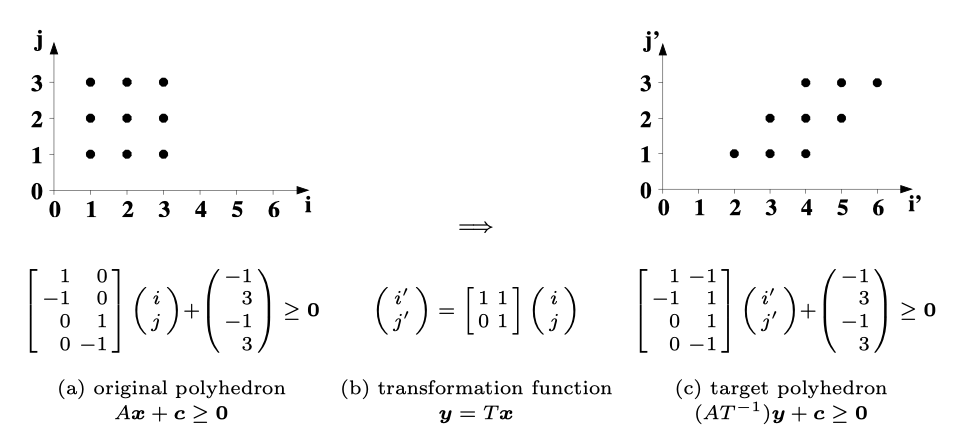
\includegraphics[scale=0.45]{images/a_skewing_transformation.png}
  \caption{a skewing transformation}
\end{figure}

\subsection{How dependences can be expressed exactly using linear (in)equalities ?}

A convenient wany to represent the scheduling constraints between the program
operations is the \textbf{\textit{Dependence Graph}}. In this directed graph:
\begin{enumerate}
  \item {\color{red} Each} program statement is represented using a
  unique vertex;
  \item The existing dependence relations between statement instances are represented
  using edges.
  \begin{itemize}
    \item {\color{red} Each vectex is labelled with the iteration domain} of the
    corresponding statement
    \item {\color{red} Each edges is labelled with the dependence polyhedra} which
    describes the dependence relation between the source and destination statements.
  \end{itemize}
\end{enumerate}

A statement $R$ \textbf{\emph{depends}} on a statement $S$ (written S$\delta$R)
if there exits an operation $S(\bm{x}_1)$, an operation $R(\bm{x}_2)$ and a memory
location $m$ such that:
\begin{enumerate}
\item $S(\bm{x}_1)$ and $R(\bm{x}_2)$ refer the same memory location $m$,
and at least one of them writes to that location.
\item $\bm{x}_1$ and $\bm{x}_2$ respectively belong to the iteration domain $S$ and $R$;
\item in the original sequential order, $S(\bm{x}_1)$ is executed before $R(\bm{x}_2)$.
\end{enumerate}

From this definition, it is easy to describe the \textbf{\emph{dependence polyhedra}} of
{\color{red}{each}} dependence relation between two statements with affine
(in)equalities. Such a dependence system has following components:

\begin{enumerate}
  \item \emph{Same memory location}: $F_S\bm{x}_S + a_S = F_R\bm{x}_R + a_R$;
  \item \emph{Iteration domains}: $A_S\bm{x}_S+\bm{c}_S\ge \bm{0}$ and  $A_R\bm{x}_R+\bm{c}_R \ge \bm{0}$;
  \item \emph{Precedence order}: $P_S\bm{x}_S - P_R\bm{x}_R + \bm{b} \ge \bm{0}$;
  \iitem this constraint can be separated into a disjunction of as many parts as there are common loops to both $S$ and $R$.
  \iitem each case corresponds to a common loop depth, and is called \emph{dependence level}.
\end{enumerate}

\begin{figure}[ht]
  \centering
  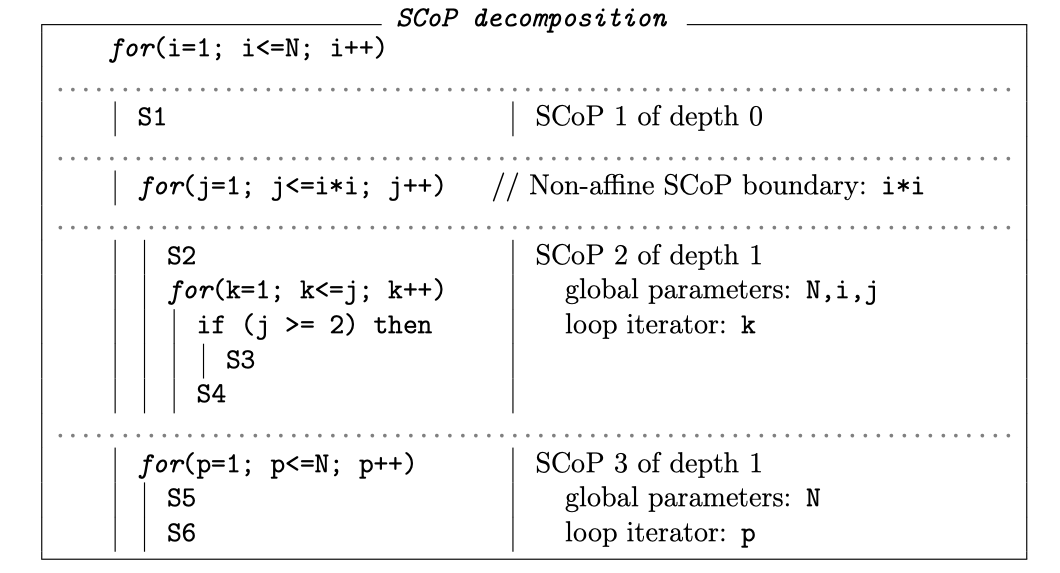
\includegraphics[scale=0.40]{images/SCoP_decomposition.png}
  \caption{SCoP decomposition}
\end{figure}

\subsection{Legal Transformation Space}

Consider the transformations as scheduling functions, \underline{the time interval
in the target program} between the executions of two operations $R(\bm{x}_R)$
and $S(\bm{x}_S)$ is:

\begin{equation}
\triangle_{R,S}\left(\begin{matrix}\bm{x}_S \\ \bm{x}_R \end{matrix} \right) =
\theta_R(\bm{x}_R) - \theta_S(\bm{x}_S).
\end{equation}

If $\mathcal{D}_{S\delta R}$ is not empty, then:
\begin{equation}
\triangle_{R,S}\left(\begin{matrix}\bm{x}_S \\ \bm{x}_R \end{matrix} \right) - \bm{1} \ge \bm{0} \label{legal}.
\end{equation}

The affine scheduling function can be expressed in terms of $D$ and $\bm{d}$ by
applying Farkas Lemma.
\begin{figure}[ht]
  \centering
  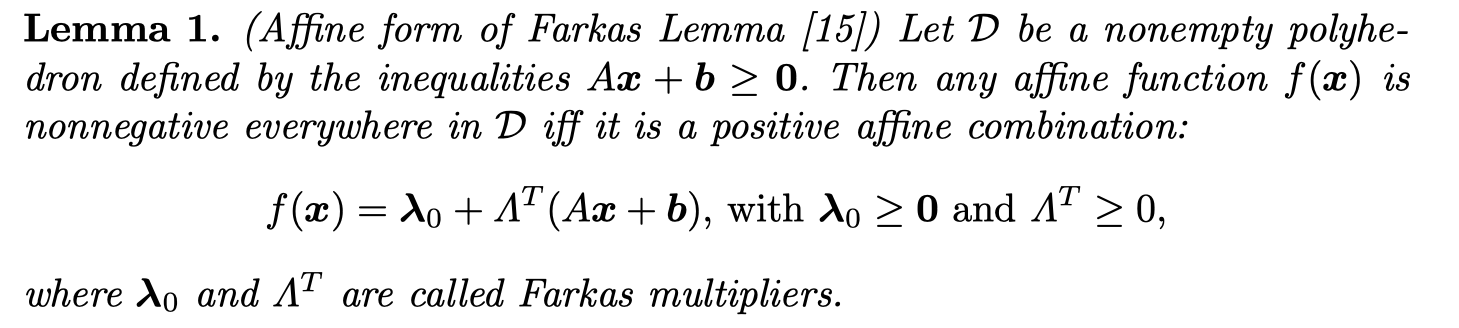
\includegraphics[scale=0.25]{images/farkas_lemma.png}
  \caption{Affine form of Farkas Lemma.}
\end{figure}

According to this Lemma, {\color{red}{for each edge in the dependence graph}},
we can find a positive vector $\bm{\lambda}_0$ and matrix $\bm{\Lambda}^T$ such that:

\begin{equation}
  T_R\bm{x}_R+\bm{t}_R - (T_S\bm{x}_S+\bm{t}_S) -\bm{1} = \bm{\lambda}_0 +
  \bm{\Lambda}^T \left( D \left( \begin{matrix}\bm{x}_S \\ \bm{x}_R \end{matrix} \right) + \bm{d} \right),
  \bm{\lambda}_0 \ge \bm{0}, \bm{\Lambda} \ge \bm{0}
\end{equation}

\subsection{Properties}

\begin{itemize}
  \item There is self-temporal reuse when $\bm{x}_r \in \text{ker}F$.
  \item The resue can be exploited \underline{if the transformed
  iteration order follows one of the reuse directions}.
  \item ({\color{red}{\textbf{??}}})\emph{Then we have to find an orthogonal
  vector to the chosen reuse direction to be the first part of the transformation
  matrix $T$.}
  \item If this partial transformation do not violate dependences, we have many choices
  for the completion procedure\footnote{I do not understand what is the completion
  procedure here? The author refers to \cite{griebl1998code} which explains completion
  to a unimodular transformation matrix.} ({\color{red}{\textbf{??}}}).
  \item To generalize, it is easy to consider not only a reuse direction vector,
  but a reuse direction space.
  \underline{\emph{in order for the transformation function to be instance-wise}}.
\end{itemize}

\section{Finding Legal Transformations}

\textbf{\textit{TBD}}


\section{Some useful reading}
\begin{enumerate}
  \item Complex transformations such as Tiling canbe achieved using linearning transformations\cite{xue1997tiling}.
  \item there is a wide range of existing data locality improvement methods,
  for the single processor case as well as compiling techniques for parallel
  systems, a well-known method is using space-time mappings\cite{lengauer1993loop}.
\end{enumerate}
